\subsection{Fundamentals of linear systems}

A linear dynamical system of states $x\in\mathbb{R}^{n}$ is simply denoted in matrix form as $\dot{x}=\mathbf{A}x$, where $\mathbf{A}$ provides the dynamics. If an action $u\in\mathbb{R}^{m}$ is taken to control the system one might write it as $\dot{x}=\mathbf{A}x+\mathbf{B}u$. In this section we are mostly interested in the first formulation (without control) for which a general solution is $x(t)=\exp(\mathbf{A}t)x(0)$, where $\exp(\mathbf{A}t)$ is a matrix given by the Taylor series expansion:

\begin{equation}
\exp(\mathbf{A}t)=\mathbf{I}+\mathbf{A}t+\frac{\mathbf{A}^2t^2}{2!}+\frac{\mathbf{A}^3t^3}{3!}+\dots+\frac{\mathbf{A}^kt^k}{k!}
\end{equation}

Evaluation of this expression is non-trivial and good precision would require a large number of terms in the expansion. For linear systems the uncoupling of equations can be done through the eigenvalues and eigenvectors of $\mathbf{A}$ obtained by solving $\mathbf{A}\xi=\lambda\xi$. If we assembly a diagonal matrix $\mathbf{D}$ with eigenvalues and the column space of eigenvectors $\mathbf{T}$ as follows

\begin{equation}
\mathbf{D}=
\begin{bmatrix}
\lambda_{1} & & & \\
& \lambda_{2} & & \\
& & \ddots & \\
& & & \lambda_{n}
\end{bmatrix}
\qquad\text{and}\qquad
\mathbf{T}=
\begin{bmatrix}
\xi_{1} & \xi_{2} & \dots & \xi_{n}
\end{bmatrix}
\end{equation}

\noindent{}then we have $\mathbf{A}\mathbf{T}=\mathbf{T}\mathbf{D}$, which is easy to proof given the eigenvalue problem definition. We can use $\mathbf{T}$ to perform the transformations $x=\mathbf{T}z$ and $\dot{x}=\mathbf{T}\dot{z}$ from which the linear dynamical system can be written as $\mathbf{T}\dot{z}=\mathbf{A}\mathbf{T}z$ or reformulated as $\dot{z}=\mathbf{T}^{-1}\mathbf{A}\mathbf{T}z$. Since $\mathbf{D}=\mathbf{T}^{-1}\mathbf{A}$, the dynamics is fully uncoupled, \emph{i.e.} all equations become independent, and stated as $\dot{z}=\mathbf{D}z$. The solution of this system takes the same form as the coupled version, but now the evaluation of $\exp(\mathbf{D}t)$ which replaces $\exp(\mathbf{A}t)$ is a simple matrix as in

\begin{equation}
\exp(\mathbf{D}t)=
\begin{bmatrix}
	\exp(\lambda_{1}t) & & & \\
	& \exp(\lambda_{2}t) & & \\
	& & \ddots & \\
	& & & \exp(\lambda_{n}t)
\end{bmatrix}
\end{equation}

Reverting the solution back to physical space $x$ is quite simple. First we note that $\mathbf{A}=\mathbf{T}\mathbf{D}\mathbf{T}^{-1}$ what can be used to show that $\mathbf{A}^{k}=\mathbf{T}\mathbf{D}^{k}\mathbf{T}^{-1}$. This property can be used to demonstrate that $\exp(\mathbf{A}t)=\mathbf{T}\exp(\mathbf{D}t)\mathbf{T}^{-1}$. Thus, the problem solution can be rewritten as $x(t)=\mathbf{T}\exp(\mathbf{D}t)\mathbf{T}^{-1}x(0)$. By the definition of $z$ we have that $z(0)=\mathbf{T}^{-1}x(0)$, then $x(t)=\mathbf{T}\exp(\mathbf{D}t)z(0)$, but $z(t)=\exp(\mathbf{D}t)z(0)$ from which one finds the solution $x(t)=\mathbf{T}z(t)$.

\subsection{Stability of linear systems}

The main take from previous section is that the key features of a linear system dynamics is encoded in matrix $\mathbf{D}$, while eigenvectors in $\mathbf{T}$ are responsible by \emph{mixing modes} to produce the response in physical space. In fact, it is the exponential behavior $\exp(\lambda_{n}t)$ of eigenvalues $\lambda_{n}$ placed over the diagonal of $\mathbf{D}$ that tell us whether values the grows indefinitely (unstable) or converges to some bounded state (stable). These eigenvalues are in the more general case complex numbers denoted as $\lambda_{n}=a_{n}\pm{}ib_{n}$. Thus, the exponential term is expanded as

\begin{equation}
\exp(\lambda_{n}t)=\exp(a_{n}t)\left[\cos\left(b_{n}t\right)\pm{}i\sin\left(b_{n}t\right)\right]
\end{equation}

From this expression we see that the complex part of solution \begin{inparaenum}[(i)]\item comes in pairs of complex conjugates, and, more importantly \item is intrinsically bounded by trigonometric functions and determine oscillatory behavior of solution. \end{inparaenum} Thus, it is the sign of $\mathbb{R}(\lambda_{n})=a_{n}$ that determines the solution stability. For any $a_{n}>0$ one of the modes in eigenspace grows indefinitely and the transformation to physical space produces an unbounded solution for $x(t)$. If all $a_{n}<0$, then the system is unconditionally stable. In Figure~\ref{fig:stability-linear-system-ct} we depict in gray the area (that extends to infinity towards negative $\Re(\lambda)$ and $\Im(\lambda)$) where eigenvalues $\lambda_{n}$ of $\mathbf{A}$ produce stable solutions to the linear system.

\begin{figure}[h!]
\centering%
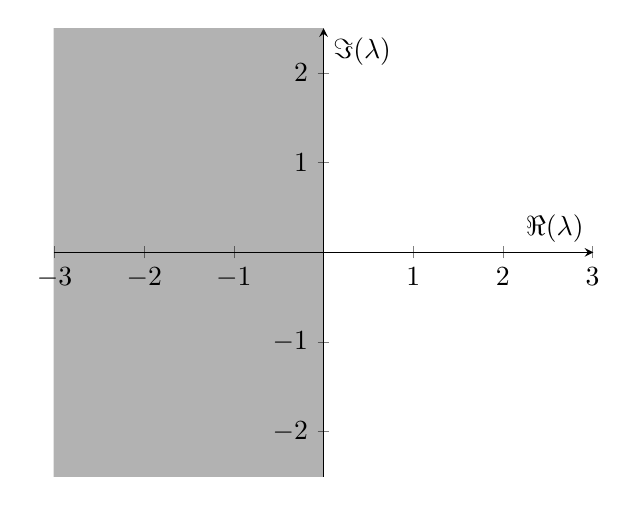
\begin{tikzpicture}
\begin{axis}[
    xmin=-2.0,
    xmax=2.0,
    ymin=-2.5,
    ymax=2.5,
    axis equal,
    axis lines=middle,
    xlabel=$\Re(\lambda)$,
    ylabel=$\Im(\lambda)$,
    disabledatascaling
]
\fill [opacity=0.3] (0.0,2.5) rectangle (-3.5,-2.5);
\end{axis}
\end{tikzpicture}
\caption{\label{fig:stability-linear-system-ct}Stability region of a linear system in continuous time.}
\end{figure}

In practice, measurements and controls are performed at discrete time points. In this case we are interested in the problem formulation in \emph{discrete time}. Representing a given solution step by index $i$, we have that $x(i+1)=\tilde{\mathbf{A}}x(i)$. It is simple to show that $\tilde{\mathbf{A}}=\exp(\mathbf{A}\tau)$, where $\tau$ is the sampling interval. Applying the time-stepping relationship recursively we find that at the $k-$th time step the solution can be expressed as $x(k)=\tilde{\mathbf{A}}^{k}x(0)$.

To investigate the stability in discrete time, we apply the same transformation as done in previous section but now applied to $\tilde{\mathbf{A}}$. This matrix can be rewritten as $\tilde{\mathbf{A}}=\tilde{\mathbf{T}}\tilde{\mathbf{D}}\tilde{\mathbf{T}}^{-1}$ from which one can show again that $\tilde{\mathbf{A}}^{k}$ depends only on $\tilde{\mathbf{D}}^{k}$. Writing the eigenvalues of $\tilde{\mathbf{D}}$ in exponential form $\lambda_{n}=R_{n}\exp(i\theta)$ leads to $\lambda_{n}^{k}=R_{n}^{k}\exp(ik\theta)$. In this expression, the exponential part is again related to oscillatory behavior only and the absolute value $R_{n}$ governs stability. Thus we conclude that in discrete time the unconditional stability arises when all $R_{n}<1$. This region is depicted in complex plane in Figure~\ref{fig:stability-linear-system-dt}.

\begin{figure}[h!]
\centering%
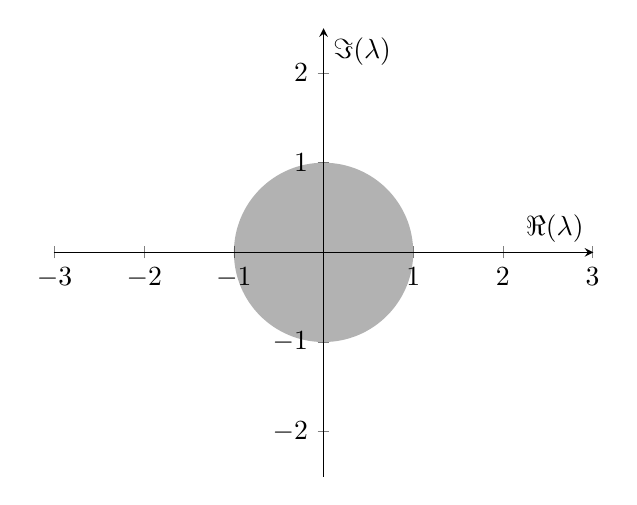
\begin{tikzpicture}
\begin{axis}[
    xmin=-2.0,
    xmax=2.0,
    ymin=-2.5,
    ymax=2.5,
    axis equal,
    axis lines=middle,
    xlabel=$\Re(\lambda)$,
    ylabel=$\Im(\lambda)$,
    disabledatascaling
]
\fill [opacity=0.3] (0,0) circle [radius=1];
\end{axis}
\end{tikzpicture}
\caption{\label{fig:stability-linear-system-dt}Stability region of a linear system in discrete time.}
\end{figure}

\endinput